\begin{abstract}
AdaptoFlux is a representation substrate for composing typed numerical operations and stateful actions in executable graphs. A metadata-driven Method Pool supplies typed interfaces, while a Generalized Data Flow Graph (GDFG) represents data reuse and per-step computation. External state connects successive graph executions. We make the execution contract explicit: a persistent program order and resource-based control dependencies determine conflicting state accesses while retaining parallelism between independent operations. The representation supports both discrete structure search and parameter optimization. In a controlled stateful synthesis experiment with identical operator implementations, fine-grained, role-merged, and flat type declarations achieve strict success in 29/30, 15/30, and 1/30 runs. A paired translation audit matches implicit and explicit state execution across 70,670 environment steps. Fixed-depth execution measurements cover up to 1,024 operation nodes and 2,176 edges. A shared-feature action controller supplies a concrete example: learned action scores feed an exclusive router, and its adapted GDFG matches a frozen controller for 20,480 steps. Further experiments examine operator-pool expansion and sustained execution in a continual-learning application. Together, these results characterize how typed composition, state ordering, and optimization interact in one executable representation.
\end{abstract}

\section{Introduction}
\label{sec:introduction}
Symbolic program synthesis searches over discrete executable structures. Its representation determines which operations can be composed, where intermediate results can be reused, and how a program interacts with mutable state. These choices matter for control tasks: a controller must combine numerical computation with observations, action selection, and environment updates, often over many successive steps. AdaptoFlux makes these interfaces explicit through a typed Method Pool and Generalized Data Flow Graphs (GDFGs).

Consider an action controller that reads an observation $o_t$ and an internal state $h_t$, computes shared features $z_t$, scores each available action, and executes the action selected by an exclusive router. One feature can contribute to several action scores without being recomputed. The state-update branch commits $h_{t+1}$ after reading $h_t$, and the same stored graph runs at the next step. This structure combines typed dataflow, learned numerical parameters, and stateful effects in a single program (Figure~\ref{fig:action_structure}).

\begin{figure}[t]
\centering
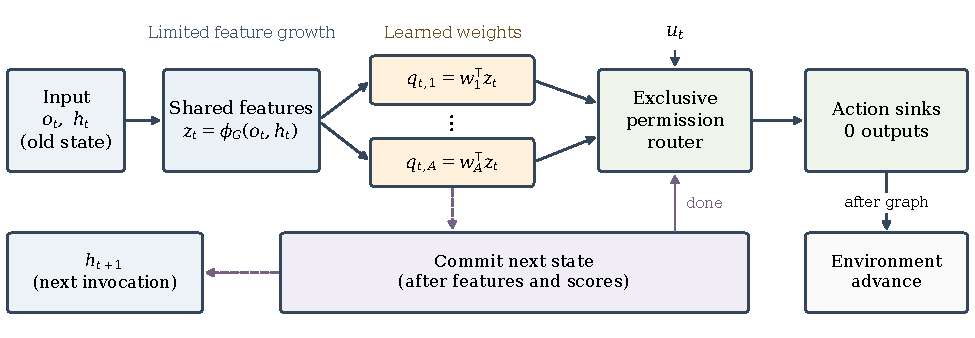
\includegraphics[width=\linewidth]{images/rebuttal_revision/action_structure.pdf}
\caption{A concrete GDFG controller. Shared features feed per-action scores; an exclusive router activates one action. The state branch reads the old state and commits the next state. Dashed purple paths show commit/control relations. The template supplies these interfaces, CMA optimizes score coefficients, and scheduled proposals can extend the feature graph.}
\label{fig:action_structure}
\end{figure}

The representation separates three decisions. \emph{Type signatures} define admissible data connections. \emph{Execution contracts} define how nodes access shared resources. \emph{Search procedures} select structures and parameters. This distinction permits several optimizers to use the same graph interface and prevents a search preference from being mistaken for a runtime guarantee. In particular, a data DAG gives a partial order: two independent data branches can still write the same external state. We therefore represent their selected state-access order explicitly.

The paper makes four contributions. First, it specifies a common registration and execution interface for typed operations, reusable subgraphs, and actions. Second, it formalizes stateful execution using a fixed program order and additional control dependencies, implemented consistently across training, inference, and model persistence. Third, controlled experiments quantify the effect of semantic type declarations, compare implicit and explicit state encodings, and measure execution costs as graph size increases. Fourth, a parameterized action-controller example and larger application studies demonstrate how the substrate supports different optimization and reuse workflows. LayerGrow, GraphEvo, and the CMA-based controller optimizer provide distinct navigation procedures for this shared representation.

The implementation is available through the anonymous review repository at \url{https://anonymous.4open.science/r/AdaptoFlux-CF54}. Protocols and the provenance of the supplementary measurements are specified in Appendices~\ref{app:revision_effects}--\ref{app:revision_capacity}.

\section{Positioning and Related Work}
\label{sec:positioning}
Typed program composition, graph reuse, and effect ordering have substantial prior foundations. Strongly typed genetic programming constrains compositions through types~\cite{montana1995strongly}; Cartesian Genetic Programming provides graph-based reuse~\cite{miller2015cartesian}; and MT-CGP explicitly supports mixed data types~\cite{harding2012mtcgp}. LLVM SelectionDAG combines typed dataflow with chain dependencies for side-effect ordering~\cite{llvmSelectionDAG}. These precedents motivate our distinction between data edges and control dependencies.

AdaptoFlux brings these mechanisms together as a runtime-facing substrate for symbolic synthesis: a registry accepts heterogeneous Python operations, a graph exposes typed data ports, external-state operations share the execution interface, and synthesized subgraphs can be registered as methods. Search procedures operate on this interface. DreamCoder studies learned reusable abstractions in a functional language~\cite{ellis2021dreamcoder}; Popper combines logical background knowledge with failure-driven constraint learning~\cite{cropper2021learning}; symbolic-policy and language-model-guided discovery emphasize search quality~\cite{landajuela2021discovering,romera2024mathematical}. These approaches offer complementary optimization and abstraction mechanisms. Our experiments characterize the executable representation and its interaction with concrete optimizers. A possible future extension is to use a language model to propose candidates for the same execution and evaluation interface (Appendix~\ref{app:llm_candidate_generation}). Appendix~\ref{sec:related_work} develops the comparisons; Appendix~\ref{sec:appendix_baseline_comparison} reports the static symbolic-regression benchmarks against gplearn and PySR~\cite{cranmer2023interpretable}.

\section{System Architecture}
\begin{figure}[t]
\centering
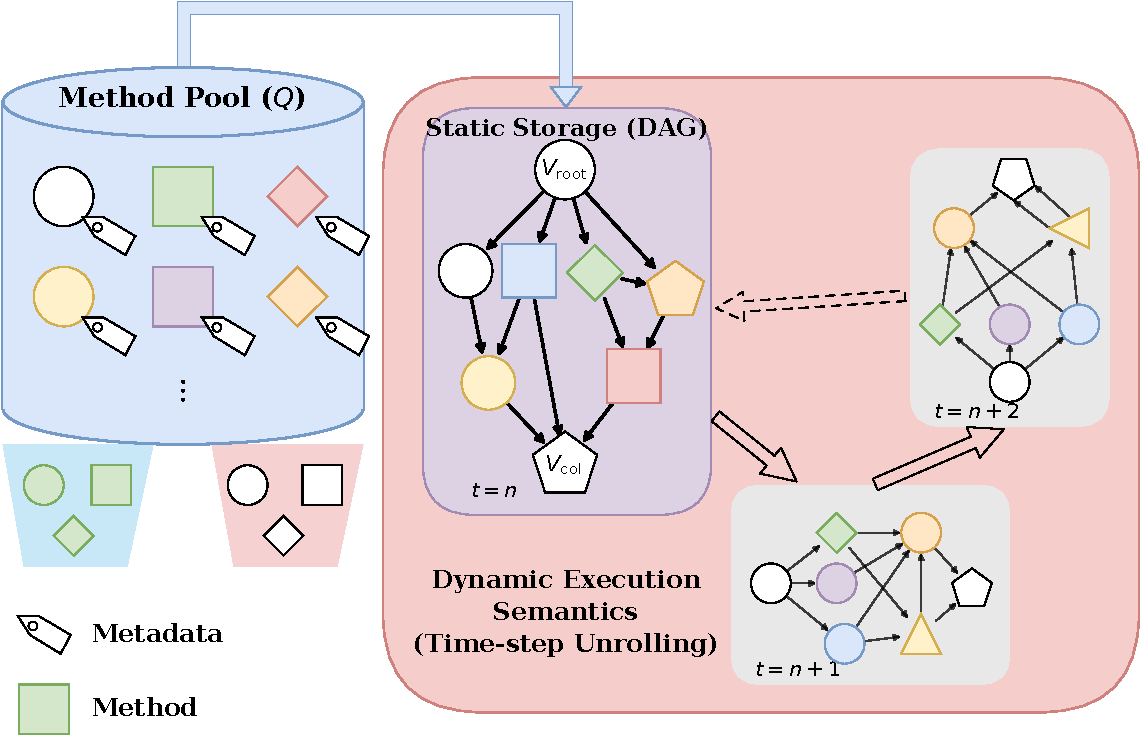
\includegraphics[width=0.74\linewidth]{images/rebuttal_format/NAD.pdf}
\caption{AdaptoFlux architecture. The Method Pool defines callable interfaces, the stored GDFG carries data dependencies, and the runtime connects successive steps through state. Effect-ordering plans add control dependencies to the per-step schedule.}
\label{fig:adaptoflux_arch}
\end{figure}

\subsection{Method Pool}
\label{subsec:method_pool}
A method is registered as $m=\langle\mathrm{impl},\sigma_{\mathrm{in}},\sigma_{\mathrm{out}},\mathrm{M}\rangle$, comprising its implementation, positional input and output type signatures, and metadata. Types are declared atoms, such as \texttt{scalar}, \texttt{pos\_type}, or \texttt{target\_type}. Each input position lists the atoms it accepts; each output port declares the atom it emits. Arity and positional routing determine which outputs can supply which inputs.

Metadata has two roles. Search annotations, including groups and sampling weights, select a view $\mathrm{Q}_{\mathrm{view}}\subseteq\mathrm{Q}$ of the pool. Execution annotations declare the resources a method reads and writes, denoted $R_m$ and $W_m$, or identify a method as pure. Undeclared effects are treated conservatively as unknown. The same resource name must describe accesses to the same external state. A registry entry can also contain a reusable subgraph; its effect contract aggregates those of its constituents. Appendix~\ref{app:metadata_role} separates these execution contracts from search preferences.

\subsection{GDFGs and Stateful Execution}
\label{sec:gdfg}
A data graph $G=\langle V,E_d\rangle$ is a DAG with input, operation, and output-aggregation interfaces. Every operation node is bound to a registered method. An edge connects a particular output port to a particular input position, and is admissible when its emitted type belongs to that position's accepted type set. The data-graph hypothesis class is
\begin{equation}
\label{eq:expression_space}
\Omega_{\mathrm Q,\Sigma}=\{G:\ G\text{ is a DAG},\ m_v\in\mathrm Q,
\text{ and every data edge respects its port types}\}.
\end{equation}
Declared type compatibility is checked during graph construction. The declarations are callable interface contracts: method implementations must also respect their declared inputs and outputs.

\paragraph{State transitions require a selected order.}
For fixed input $x_t$, a node computes data outputs and may update the current external state. Let $\pi=(v_1,\ldots,v_m)$ be a selected topological order. Writing $F_v$ for the state component of node execution, one step is
\begin{equation}
\label{eq:state_transition}
s^{(0)}=s_t,\qquad
s^{(k)}=F_{v_k}(\mathbf{in}_{v_k},s^{(k-1)},x_t),\qquad
s_{t+1}=s^{(m)}.
\end{equation}
The choice of $\pi$ matters. Starting from $s=1$, independent nodes that apply $s\leftarrow s+1$ and $s\leftarrow2s$ produce either $4$ or $3$. Both orders may satisfy the same data DAG. We therefore define the stateful executable program by $P=(G,\pi,E_c)$, where $E_c$ contains control dependencies that preserve the selected order of conflicting accesses.

\paragraph{Conflict-aware scheduling.}
Two nodes conflict when
\begin{equation}
W_u\cap(R_v\cup W_v)\ne\varnothing
\quad\text{or}\quad W_v\cap R_u\ne\varnothing.
\end{equation}
For each conflicting pair with $u\prec_\pi v$, the augmented graph $G^+=(V,E_d\cup E_c)$ contains a dependency path from $u$ to $v$. The implementation constructs these paths using resource read/write frontiers; control dependencies carry completion information, while function arguments come only from $E_d$. Shared reads and accesses to disjoint resources remain available for parallel execution. Unknown methods are conservatively ordered with other effectful methods.

With complete effect declarations, deterministic operations, the same inputs and initial state, and successful execution, legal schedules of $G^+$ produce the same outputs and final state. Adjacent independent operations can be exchanged without changing their inputs or resource observations; conflicting operations retain their order. Appendix~\ref{app:revision_effects} gives the execution conditions and validation. If operation-node updates admit increments $I_v$ applied by $\oplus$, and those increments can be evaluated from the same pre-step state and commute on disjoint resources, Equation~\ref{eq:state_transition} reduces to
\begin{equation}
\label{eq:state_parallel}
s_{t+1}=s_t\oplus\bigoplus_{v\in V_{\mathrm{proc}}} I_v(\mathbf{in}_v,s_t,x_t).
\end{equation}

\paragraph{Training and persistence.}
Before a candidate is evaluated, the runtime freezes its initial order. Stable node identities retain that order through accepted substitutions, graph growth, copying, and save/load operations. An explicit order change defines a new candidate for evaluation. For effectful batches, the runtime finishes a complete sample before starting the next. The effect-ordering feature is enabled by default and can be disabled; the selected mode is stored with the model. Disabled mode follows data dependencies and node-wise batching, with no additional state-ordering guarantee.

Across time steps, external state or explicit state inputs connect successive executions of the same stored graph. A finite unrolling uses forward-in-time connections and remains acyclic (Appendix~\ref{app:runtime_loops}). The hand-written Snake example uses mutually exclusive action permits; the controller in Figure~\ref{fig:action_structure} additionally exposes a read-old/commit-new internal-state boundary.

\subsection{Navigation and Reuse}
\label{subsec:navigability_validation}
\textbf{LayerGrow} samples type-compatible operations to extend a graph, evaluates the candidate, and accepts or rolls back the extension. \textbf{GraphEvo} refines a fixed graph skeleton by replacing its bound methods, and can extract subgraphs into reusable methods. \textbf{CombinedTrainer} composes growth and refinement with pool filtering. Their algorithmic descriptions and original experiments are retained in Appendices~\ref{sec:detailed_analysis} and~\ref{sec:appendix_experiments}. The action-controller study uses CMA to optimize numerical score coefficients and scheduled proposals to grow arithmetic features, illustrating a second optimization interface on the same form of executable structure.

\subsection{Execution Cost and Parallelism}
\label{subsec:inference_complexity}
For $V$ operations, $E_d$ data edges, $E_c$ control edges, batch size $N$, and average operation cost $\bar C_{\mathrm{op}}$, inference separates plan preparation, scheduling, routing, and computation:
\begin{equation}
T_{\mathrm{infer}}=T_{\mathrm{prepare}}+T_{\mathrm{sched}}(N,G^+)
+O\bigl(N(|E_d|C_{\mathrm{route}}+V\bar C_{\mathrm{op}})\bigr).
\end{equation}
The revised runtime validates the graph and reconstructs its plan on each call. Pure graphs use one batched traversal, whereas effect-ordered stateful batches use $N$ complete traversals. The threaded implementation sorts ready nodes and creates a worker pool for each traversal; these costs belong to $T_{\mathrm{sched}}$. Resource declarations and the selected ordering determine preparation and control bookkeeping. The historical backend's measurements and complexity breakdown are given in Appendix~\ref{sec:complexity_analysis}.

Parallel benefit depends on the ready graph width, critical path, operation cost, and backend. The original simulated non-blocking workload achieved a mean $10.25\times$ speedup with 16 workers. The supplementary Python scalar CPU workload instead runs faster serially (Section~\ref{subsec:execution_scaling}). Reporting both regimes distinguishes available graph concurrency from the cost of realizing it.

\subsection{Search-Space Structure}
\label{subsec:search_complexity}
Type routing removes inadmissible port compositions before evaluation. Search annotations then select among admissible candidates; effect contracts determine their execution. Increasing the pool can introduce useful operations and simultaneously increase the choices explored under a fixed budget. LayerGrow's cost accumulates across repeated graph extensions, while GraphEvo refinement holds the skeleton fixed. The experiments below measure these effects separately from execution scalability.

\section{Experimental Results}
\label{sec:experiments}
We report three evidence groups: the original navigation experiments, supplementary controlled measurements, and applications developed with additional optimizers. The four supplementary studies of type priors, state encoding, execution scaling, and controller replay used the original frozen ATF backend. The revised effect-aware runtime has a separate regression suite and frozen-model replay audit. Appendix~\ref{app:revision_effects} records this version separation.

\subsection{Structural Search with LayerGrow}
\label{subsec:layergrow_validation}
On Titanic~\cite{titanic}, LayerGrow uses nine scalar operations and a 2,500-attempt budget per run. Across ten runs per maximum-layer setting, mean best accuracy reaches $0.763\pm0.041$ at a configured maximum of 20 layers. Higher requested maxima produce little further improvement (means 0.769--0.783 for settings 25--50) and more budget exhaustion. At requested maxima 45 and 50, all runs exhaust the attempt budget; the mean reached depths are 19.6 and 18.7. Thus the observed failure concerns this growth procedure's progress under its budget. Figure~\ref{fig:scaling_behavior} and Appendix~\ref{sec:appendix_exp1} give the full depth and cost results.

\subsection{GraphEvo and Reusable Subgraphs}
\label{subsec:graphevo_validation}
The task chain $f_1(x)=2(x+1)$, $f_2(x)=f_1(x)+3$, and $f_3(x)=0.5f_2(x)$ evaluates whether extracted structure can support a later task. Under the controlled two-layer setting, evolved methods yield Task~3 success in 13/100 runs, compared with 0/100 without evolution and 12/100 with a hand-supplied prior. The three-layer setting yields 9/100. Extraction enables reuse under the chosen initialization constraints, while deeper initialization changes the search difficulty. Appendix~\ref{sec:appendix_exp2} reports all conditions and Figure~\ref{fig:exp3_chain} separates partial and complete transfer chains.

\subsection{Semantic Type Priors in Stateful Synthesis}
\label{subsec:stateful_synthesis}
The supplementary Minimal Stateful Attractor experiment holds nine operator implementations fixed and varies only their declared types. The conditions distinguish position and target roles, merge them into one quantity type, or represent all values as scalars. Each condition uses the same 30 search seeds. Each evaluation exhaustively tests the 20 unequal start/target pairs in $\{-2,-1,0,1,2\}$, with at most four graph steps per episode. Strict run success requires solving all 20 pairs.

\begin{table}[t]
\centering
\caption{Semantic type priors improve stateful synthesis. All conditions use the same nine operator bodies and nominal search caps. Evaluation calls report the realized cost; intervals are Wilson 95\% intervals across 30 runs.}
\label{tab:revision_type_main}
\small
\begin{tabular}{lrrr}
\toprule
Type declarations & Successful runs & 95\% interval & Mean calls \\
\midrule
Position / target & 29/30 (96.7\%) & 83.3--99.4\% & 59.47 \\
Merged quantity & 15/30 (50.0\%) & 33.2--66.8\% & 81.67 \\
All scalar & 1/30 (3.3\%) & 0.6--16.7\% & 738.67 \\
\bottomrule
\end{tabular}
\end{table}

Table~\ref{tab:revision_type_main} shows a clear contribution from semantic role information: merging position and target types reduces success from 29 to 15 runs, and flattening all types reduces it to one. Initialization already solves 20, 4, and 0 runs, respectively; refinement supplies the remaining successes. Type declarations improve both the initial candidate distribution and the set of permitted replacements. The realized evaluation budgets differ because stopping conditions and available replacements differ. Appendix~\ref{app:revision_types} reports these budgets, seed-level outcomes, and final-model audits. The original 10-seed experiment, which used a different evaluation protocol and obtained 8/10 versus 0/10, is retained separately in Appendix~\ref{sec:appendix_exp4}.

\subsection{Execution Consistency under Alternative Schedules}
\label{subsec:execution_consistency}
The revised executor preserves each evaluated candidate's selected state-access order through acceptance, copying, and model reloads. Structural edits produce candidates for evaluation; serial and threaded executions of a fixed candidate agree. We evaluate this at two levels. First, targeted tests exercise non-commuting writes, read/write conflicts, disjoint resources, unknown effects, and zero-output action nodes. Second, the 90 final models from the type experiment are replayed on all 20 initial conditions in serial and three-worker modes. Every trajectory and saved loss/accuracy value agrees, covering 1,800 model--initial-state pairs and 4,934 paired environment steps (Table~\ref{tab:runtime_consistency_main}).

\begin{table}[tb]
\centering\small
\caption{Execution consistency of the revised runtime. Graph-level replay uses frozen models; targeted tests separately exercise scheduling and persistence behavior.}
\label{tab:runtime_consistency_main}
\begin{tabularx}{\linewidth}{@{}lX@{}}
\toprule
Validation & Observed result \\
\midrule
Models / model--initial-state pairs & 90 / 1,800 \\
Serial versus three-worker replay & All 4,934 paired steps match \\
Saved evaluation metrics & All accuracy and loss values match \\
Small mixed-resource graph & All legal schedules preserve state and reads \\
Independent-branch synchronization test & Confirms actual concurrent execution \\
Implementation regression suite & 85 tests and 46 subtests pass \\
\bottomrule
\end{tabularx}
\end{table}

The mixed-resource test enumerates every legal topological schedule of a six-operation graph containing independent resources and conflicting accesses. A separate randomized check compares inferred control dependencies against 150 resource-access configurations. The synchronization test uses a barrier inside independent methods: both workers must enter before either completes. This confirms that consistency is achieved while retaining available concurrency. For a chain of 250 methods with unknown effects, the plan requires 249 control edges, demonstrating the frontier construction's compact treatment of conservative ordering.

The persistence tests reorder stored nodes and edges and preserve stable node identities. Loaded programs retain their evaluated order and resource declarations. Training tests cover candidate acceptance, rollback, graph growth, and composite-method extraction. Together, the replay and targeted tests connect the execution contract in Section~\ref{sec:gdfg} to the paths used by training and deployment. Appendix~\ref{app:revision_effects} specifies the complete contract and the optional execution modes.

\subsection{Implicit and Explicit State Encodings}
For each of 1,007 candidate/final-model records, we translated implicit state accesses into immutable explicit-state inputs and outputs while preserving the selected access order. Across 20,140 paired initial conditions and 70,670 paired environment steps, node values, state transitions, trajectories, and final metrics agree. This establishes an operational correspondence between the two encodings for the evaluated programs.

The explicit encoding adds an average of 2.189 state edges over the 90 final graphs and no operation nodes. Its paired execution-time ratio relative to the implicit implementation has median 1.137, including state-object construction and adapter dispatch. Table~\ref{tab:encoding_main} summarizes the correspondence.

\begin{table}[tb]
\centering\small
\caption{Matched state encodings on the original executor. Records include repeated final graphs; timing summarizes 90 final models with five paired repetitions per model.}
\label{tab:encoding_main}
\begin{tabular}{lr}
\toprule
Comparison quantity & Result \\
\midrule
Graph records / paired initial conditions & 1,007 / 20,140 \\
Paired environment steps & 70,670 \\
Numerical values, state, trajectories, metrics & All matched \\
Additional operation nodes & 0 \\
Mean additional state edges & 2.189 \\
Explicit/implicit time ratio: median [quartiles] & 1.137 [1.086, 1.197] \\
\bottomrule
\end{tabular}
\end{table}

The translation gives every state-reading or state-writing operation an immutable $(p,g)$ token input and output. Token edges follow the original access order, and a final edge returns the new state. Numerical argument binding and output aggregation are unchanged. During the explicit run, the unrelated implicit global state is deliberately altered; explicit outputs remain unchanged and that global state is not modified. This check verifies that state dependence has moved into the graph ports rather than remaining hidden in the method wrappers. The two implementations thus expose the same transition through different interfaces: shared external resources in one, explicit state values in the other. Appendix~\ref{app:revision_encoding} details the translation and timing protocol.

\subsection{Scaling Graphs, Pools, and Execution Workloads}
\label{subsec:execution_scaling}
\paragraph{Single-graph execution.}
At fixed depth eight and batch size 32, we vary width to obtain 32--1,024 operation nodes and 68--2,176 edges, with five graph seeds at each size. Serial time increases from 2.127 to 70.586\,ms across this 32-fold node increase. At the largest size, a separate declared-type compatibility pass takes 1.448\,ms and topological preparation takes 2.310\,ms. Four-worker time is 82.379\,ms: threading is slower for these Python scalar CPU operations. All 30 graphs agree with an independent numerical reference (maximum absolute error $2.22\times10^{-16}$). Figure~\ref{fig:revision_scaling} shows the measured curves; 1,024 nodes is the largest tested point, and the overhead-dominance threshold has not been reached in this sweep.

\begin{figure}[t]
\centering
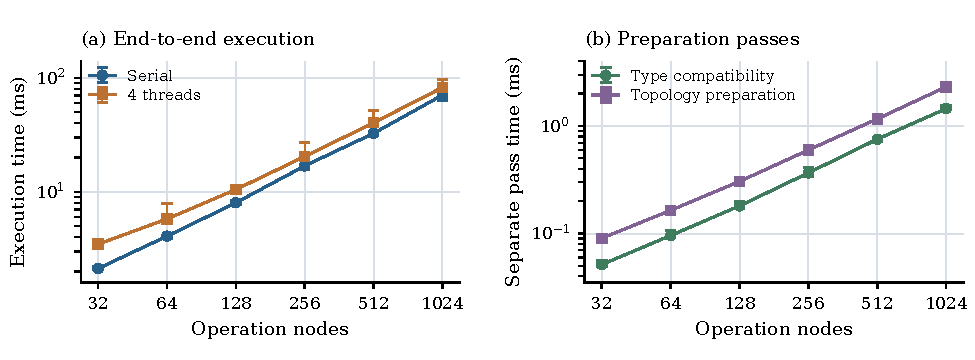
\includegraphics[width=\linewidth]{images/rebuttal_revision/execution_scaling.pdf}
\caption{Fixed-depth scaling on the original backend. Medians summarize five graph seeds per size; error bars show their minimum--maximum range. Each metric uses two warm-ups and seven repetitions. The declared-type pass and topology preparation are measured separately; inference includes its own preparation. Full measurements are in Appendix~\ref{app:revision_scaling}.}
\label{fig:revision_scaling}
\end{figure}

\paragraph{Atomic operator-pool expansion.}
A follow-on search implementation compares nine pools containing 6--20 operators across 12 numerical tasks and four action tasks. Pool expansion has a non-monotonic effect under fixed candidate and interaction budgets (Table~\ref{tab:pool_expansion_main}). The six-operation arithmetic core gives the strongest aggregate numerical pass rate along the nested expansion; adding increment, decrement, and negation gives the strongest maze result. The different responses show that useful operator coverage and the distribution of candidates jointly shape search quality.

\begin{table}[tb]
\centering\small
\caption{Nested atomic-pool expansion. Numerical pass rate averages ten task families and four seeds; maze completion averages two seeds. Both values are percentages.}
\label{tab:pool_expansion_main}
\begin{tabular}{rrr}
\toprule
Operators & Numerical input pass rate & Maze completion \\
\midrule
6 & 14.01 & 11.43 \\
9 & 11.45 & 58.01 \\
15 & 7.72 & 37.89 \\
20 & 11.35 & 6.93 \\
\bottomrule
\end{tabular}
\end{table}

Numerical conditions use 131,072 training input presentations per task and seed, 256 candidate opportunities, and a 32-node graph cap. Action conditions use 65,536 training episodes, 128 candidate opportunities, and a 24-node cap. Numerical success in the table is the fraction of test inputs with relative error at most 1\%. The extensions change operator composition and arity along with pool size. Appendix~\ref{app:revision_pool} gives the full nine-pool comparison and the path-feedback procedure. This experiment identifies a practical design choice: pool views should expose operations relevant to the task while controlling the alternatives presented to a finite-budget optimizer.

\paragraph{Sustained execution and reusable libraries.}
A continual-learning application runs 80 sequences of 40 stages across ten training seeds. Each observation has 64 fields, one of 32 identities, and six available actions. The sequence presents 20 rule families and then returns to them in reverse order. The completed runs record 9,830,400 valid training actions and 229,376,000 evaluation input rows: 239,206,400 input rows in total undergo native-ATF risk-output checks. These counts measure application workload; graph calls can process whole arrays.

\begin{table}[tb]
\centering\small
\caption{Library capacity in the 40-stage application. Costs count environment interactions and average ten paired seeds; lower is better. Return cost measures recovery of previously encountered rule families.}
\label{tab:library_main}
\begin{tabular}{lrrr}
\toprule
Configuration & Capacity & Mean attainment cost & Return cost \\
\midrule
Direct reuse & 32 & 1,792.32 & 1,749.76 \\
Direct reuse & 128 & 1,691.52 & 1,512.96 \\
Full combination & 32 & 1,855.04 & 1,802.88 \\
Full combination & 128 & 1,683.20 & 1,472.00 \\
\bottomrule
\end{tabular}
\end{table}

Attainment cost counts interactions up to the earliest checkpoint after which balanced risk accuracy of at least 90\% and optimal-action rate of at least 80\% in the carrying condition are maintained. A stage that never attains this criterion receives a cost of 3,200. Increasing capacity from 32 to 128 lowers mean attainment cost by 5.62\% for direct reuse and 9.26\% for the full configuration (Table~\ref{tab:library_main}). The full configuration's return cost decreases by 18.35\%, while its first-exposure cost changes little. Additional retained structures therefore help most when earlier tasks are revisited. At capacity 32, the full configuration does not meet its predeclared advantage criterion over direct reuse. A separate shorter capacity sweep shows no stable gain; its capacity-32 and capacity-64 runs produce identical trajectories because occupancy never exceeds 21 entries. The results distinguish retention capacity from the search and selection mechanism used with it. Appendices~\ref{app:revision_large} and~\ref{app:revision_capacity} provide all eight conditions and the short-sequence comparison.

\subsection{A Learned Action-Scoring Controller}
The structure in Figure~\ref{fig:action_structure} computes
\begin{equation}
z_t=\phi_G(o_t,h_t),\qquad q_{t,a}=\sum_j w_{a,j}z_{t,j},\qquad
a_t=\operatorname{route}(q_t,u_t).
\end{equation}
The router uses a supplied draw $u_t$ when its selection rule is stochastic. The template supplies shared features, per-action score branches, exclusive permits, zero-output action sinks, and state-update interfaces. CMA learns the score coefficients; scheduled structure proposals can add arithmetic features or change state-emission sources. Table~\ref{tab:action_main} reports held-out completion across five training seeds, with a separate model for each task.

\begin{table}[tb]
\centering\small
\caption{Held-out action-task completion (\%). Each trained model is evaluated on 2,048 episodes. Mean and range summarize five training seeds; individual results are in Appendix~\ref{app:revision_action}.}
\label{tab:action_main}
\begin{tabular}{llrrr}
\toprule
Task & Completion criterion & Step cap & Mean & Seed range \\
\midrule
Catch & Catch all 16 balls & 160 & 92.10 & 61.28--100.00 \\
Maze & Reach $(7,7)$ & 1,024 & 92.74 & 75.98--98.88 \\
Snake & Collect 8 food items & 512 & 43.55 & 0.05--93.12 \\
Bird & Pass all 32 pipes & 1,024 & 100.00 & 100.00--100.00 \\
\bottomrule
\end{tabular}
\end{table}

Bird succeeds consistently, while Snake exposes substantial training-seed variation. In the validation-selected representative system, Catch, Maze, and Snake have no subsequent feature-growth event; Bird has four. Its 44 shared features supply 88 coefficients. For example, $z_{16}=\texttt{gapBottom}+h^{\mathrm{old}}_1$ enters the flap and coast scores with weights approximately $+3.001$ and $-6.538$, directly illustrating how one state-dependent calculation serves competing action branches. Feature proposals occur at fixed training-budget milestones, so the contribution of optimized coefficients and the occurrence of structural growth can be inspected separately in the saved controller.

A frozen bird model selected by validation was adapted from 314 nodes/411 edges to 316 nodes/565 edges by making its input, state-commit, routing, and observation interfaces explicit. Running this adapted graph in the original ATF executor matches the source controller and an independent interpreter for 20,480 steps over 20 fixed test episodes, with zero difference in features, scores, state, and actions. The replay connects the learned controller to the original execution interface. Appendix~\ref{app:revision_action} gives the five-seed results and adapter specification.

The adapter exposes a complete control step: feature and score nodes read the old state; a single commit node writes the next state; a completion dependency releases the router; the selected action sink records the action; and the environment advances after graph execution. Thus shared computation, state update, and action emission each have an explicit place in the program. The example shows how the representation carries a learned numerical controller while preserving its discrete execution structure.

\section*{Limitations}
\label{sec:limitations}
The stateful synthesis task isolates a supplied semantic type prior in a small environment. A remaining comparison is independent search with an explicit-state GP/CGP system under matched realized budgets. The larger applications use additional optimizers and task templates, and their performance depends on these choices. Effect ordering relies on accurate resource declarations; arbitrary Python side effects and runtime exceptions are outside static type compatibility. New-runtime preparation overhead requires its own performance measurements. The graph sweep has not located the practical upper bound or independently varied edge density. Python CPU threading is slower in the measured scalar workload, while the restricted static symbolic-regression benchmark favors specialized solvers on several formulas. These findings identify concrete next steps in search, backend engineering, and evaluation.

\section{Conclusion}
\label{sec:conclusion}
AdaptoFlux provides a common executable interface for typed dataflow, shared computation, and stateful actions. Persistent ordering resolves ambiguous shared-state access without changing method arguments. The experiments show that semantic type roles improve stateful synthesis, matched explicit and implicit encodings preserve program behavior, and execution cost remains measurable across substantially larger graphs and sustained application workloads. The learned action-scoring example connects these mechanisms in a controller whose behavior is reproduced by the original executor. The resulting substrate supports several optimization strategies while making their type, state, and execution contracts explicit.

Our ongoing research investigates how a single continually learning agent can use AdaptoFlux to acquire executable knowledge from interaction, retaining learned computational subgraphs together with their applicability conditions and supporting evidence for reuse across tasks. We aim to use unexpectedly beneficial outcomes and contradictory feedback to guide exploration and local graph revision, allowing knowledge to accumulate and adapt as task rules change within bounded memory and computation budgets.
\label{maintext:end}
\clearpage

\subsection*{AI use statement}
AI assistants supported the revision through implementation assistance, supplementary experiment scripting, result checking, literature lookup, English drafting and editing, and figure and layout preparation. Numerical results are derived from saved execution records and analysis scripts. The software checks include matched-state replay, independent numerical references, and regression tests. The authors are responsible for the paper's claims and the verification of AI-assisted material.

\subsection*{Ethics statement}
This work follows the ICLR Code of Ethics. It uses public benchmark data and synthetic tasks, involves no human-subject intervention, and reports no personally identifiable experimental data. Automatically generated programs can invoke external actions; applications should validate registered methods and isolate execution environments. Appendix~\ref{app:broader_impacts} discusses interpretability, misuse, and bias inherited from supplied methods.

\subsection*{Reproducibility statement}
The appendices specify method pools, seeds, evaluation criteria, runtime versions, and measurement protocols. The supplementary type study retains final graphs and complete evaluation traces; the state audit retains paired trajectories; the scaling study retains per-seed repetitions and independent reference checks; and the controller case retains its frozen model and stepwise replay. The original implementation and experiment materials are linked through the anonymous repository. Additional evidence is identified by its protocol and artifact names in Appendices~\ref{app:revision_effects}--\ref{app:revision_capacity}; its execution records are kept separate from historical experiments. Data-graph type checks, effect-ordering assumptions, and finite-unrolling arguments are specified in Sections~\ref{sec:gdfg}--\ref{subsec:inference_complexity} and Appendix~\ref{app:runtime_loops}.
